\numberwithin{equation}{section}
\numberwithin{table}{section}
\newtheorem{example}{Example}
\section{Preliminaries}
\label{sec:preliminaries}
\subsection{Propositional Logic Formula}
Propositional logic formulas are Boolean combinations of atomic propositions i.e., each atomic proposition is a statement which is either $\mathbf{true}$ or $\mathbf{false}$. A well-formed propositional logic has following grammar:
$$\varphi\hspace{3mm} :=\hspace{3mm} a\hspace{3mm} |\hspace{3mm} (\neg \varphi)\hspace{3mm} |\hspace{3mm} (\varphi \wedge \varphi)$$
Here $a$ is an atomic proposition.\newline
Syntactic sugar (a syntax which make propositional logic formulas easier to read or to express) for propositional logic formulas are given below:
$$\perp\hspace{3mm}:=\hspace{3mm}(a\wedge\neg a)$$
$$\top\hspace{3mm}:=\hspace{3mm}(a\wedge\neg a)$$
$$(\varphi_{1}\vee\varphi_{2}) := \neg((\neg \varphi_{1}) \wedge (\neg \varphi_{2})) $$
$$(\varphi_{1}\rightarrow\varphi_{2}) := ((\neg \varphi_{1}) \vee \varphi_{2}) $$
$$(\varphi_{1}\leftrightarrow\varphi_{2}) := ( (\varphi_{1}\rightarrow\varphi_{2}) \wedge (\varphi_{2}\rightarrow\varphi_{1}))$$
$$(\varphi_{1}\oplus\varphi_{2}) := (\varphi_{1} \leftrightarrow (\neg \varphi_{2})) $$
We omit parentheses according to the operator following operator precedence:
\[ \xleftarrow{\hspace*{4cm}} \]
$$\neg\hspace{3mm} \wedge\hspace{3mm} \vee\hspace{3mm} \rightarrow\hspace{3mm} \leftrightarrow\hspace{3mm} $$
\begin{example}
	Some propositional logic formulas are given below:
	\begin{itemize}
	\item $(\neg a)$
	\item $((a\wedge b)\vee c)$
	\item $((a\rightarrow b)\rightarrow c)$
	\end{itemize}
\end{example}
\subsection{Conjunctive Normal Form}
A propositional logic formula is said to be in Conjunctive Normal Form (CNF) if and only if it is a conjunction of clauses, where clause is a disjunction of literals. A literal could be a positive or negative instance of Boolean variable. A CNF formula $\varphi$ is defined as follows:
$$\varphi = \bigwedge\limits_{i=1\ldots n} C_{i}$$
$$ C_{i} = \bigvee\limits_{j=1\ldots m_{i}} a_{ij}$$
Here, $C_{i}$ is the $i^{\text th}$ clause and $n$ is total the number of clauses in $\varphi$, $a_{ij}$ is a literal and $m$ is the total number of literals in $C_{i}$.\newline
\begin{example}
	\label{cnf}
	Assume the following CNF formula,
	$$\varphi=\underbrace{(x)}\limits_{C_{1}}\wedge\underbrace{(\neg x)}\limits_{C_2}\wedge\underbrace{(\neg x\vee y)}\limits_{C_{3}}\wedge\underbrace{(\neg x \vee \neg y)}\limits_{C_{4}}$$
	where, $x, \neg x, y$ and $\neg y$ are the literals.
\end{example}

The aforementioned CNF formula which is unsatisfiable will be used as an example throughout this paper.
\subsection{Satisfiability Checking}
Satisfiability checking for propositional logic determines whether a given propositional logic formula is satisfiable. One of the most successful technologies for this test is SAT solving.\newline
A SAT solver solves the above satisfiability checking problem by implementing a decision procedure. The Davis–Putnam–Logemann–Loveland (DPLL) algorithm is the basis for most modern SAT solvers. The input formula of it is expected to be in CNF. It's not possible to explain SAT solver shortly.\newline
A propositional logic formula is said to be satisfiable if it is possible to find an assignment that makes the formula $\mathbf{true}$, otherwise unsatisfiable.
\begin{example}
	Assume two propositional formulas be defined as $\varphi_{1}=x\vee y$ and $\varphi_{2}=x\rightarrow y$, $\alpha : \{x, y\}\rightarrow \{0, 1\}$ be an assignment with $\alpha (x)=1$ and $\alpha (y)=0$. Considering Table \ref{truth-table} $(0=\mathbf{false}$ and $1=\mathbf{true})$:
	\begin{table}[]
		\centering
		\caption{Truth Table}
		\label{truth-table}
		\begin{tabular}{|c|c|c|c|}
			\hline
			$x$ & $y$ & $x \vee y$ & $x\rightarrow y$ \\ \hline
			0   & 0   & 0          & 1                \\ \hline
			0   & 1   & 1          & 1                \\ \hline
			1   & 0   & 1          & 0                \\ \hline
			1   & 1   & 1          & 1                \\ \hline
		\end{tabular}
	\end{table}
	So, $\varphi_{1}$ is satisfiable for the assignment, whether $\varphi_{2}$ is unsatisfiable.
\end{example}
\subsection{Clause-Selector Variables}
The authors of the paper \cite{karem} have used clause-selector variable to augment a CNF formula. A clause-selector variable is a variable, $w_{i}$ which is negated to augment each clause $C_{i}$ of a CNF $\varphi$ such that $C^{\prime}_{i}=(\neg w_{i}\vee C_{i})$ are the clauses of the new formula $\varphi^{\prime}$. Notice that each $C^{\prime}_{i}$ is an implication, $C^{\prime}_{i}=(w_{i}\rightarrow C_{i})$. It means if $w_{i}$ is set to $\mathbf{true}$, the original clause $C_{i}$ must be satisfied. Conversely, assigning $w_{i}$ to $\mathbf{false}$ means that $C_{i}$ does not need to satisfied for satisfying $C_{i}^{\prime}$, which corresponds to removing $C_{i}$ from $\varphi$. So, adding clause-selector variables provides the SAT solver the ability to enable and disable clauses as a part of its normal search.
\begin{example}
	For our example formula $\varphi=(x)\wedge(\neg x)\wedge(\neg x\vee y)\wedge(\neg x \vee \neg y)$, after adding clause-selector variables we get the following augmented formula $\varphi^{\prime}$, 
	$$\varphi^{\prime}=(\neg w_{1}\vee x)\wedge(\neg w_{2}\vee \neg x)\wedge(\neg w_{3}\vee \neg x\vee y)\wedge(\neg w_{4}\vee \neg x \vee \neg y)$$
	
\end{example}
\subsection{Minimal Unsatisfiable Subset and Minimal Correction Subset}
An Unsatisfiable Subset (US) of $\varphi$ for an unsatisfiable CNF formula $\varphi$ is a subset of the clauses of whose conjunction is unsatisfiable. An US is said to be a Minimal Unsatisfiable Subset (MUS) if and only if removing any clause from the US makes it satisfiable. A Minimal Correction Subset (MCS) is a subset of the clauses of $\varphi$ whose removal from $\varphi$ makes it satisfiable and which is minimal.
\begin{definition}[MUS]
	\label{def:mus}
	For a propositional logic formula $\varphi$ in CNF, a subset $U$ of $\varphi 's$ clauses is an US $\emph{for $\varphi$}$ if $\bigwedge \limits_{C\in U}C$ is unsatisfiable. An US $\emph{for $\varphi$}$ is $\emph{minimal}$ (MUS) if for all $U^{\prime}\subset U, \bigwedge \limits_{C\in U^{\prime}}C$ is satisfiable.
\end{definition}
\begin{definition}[MCS]
	\label{def:mcs}
	For a propositional logic formula $\varphi$ in CNF, a subset $M$ of $\varphi 's$ clauses is an MCS $\emph{for $\varphi$}$ if $\bigwedge \limits_{C \in M}C$ is satisfiable and for all $M^{\prime}\subset M, (\varphi slashDiteHobe \bigwedge \limits_{C\in M^{\prime}}C)$ is unsatisfiable.
\end{definition}
A formula can have multiple MUSs and MCSs. For any formula $\varphi$, the set of all MUSs and MCSs of $\varphi$ are denoted by MUSs($\varphi$) and MCSs($\varphi$), respectively.
For our example formula from \ref{cnf}, the MUSs and MCSs are shown in the Table $2.1$.
\begin{table}[]
	\centering
	\caption{All MUSs and MCSs}
	\label{mus-mcs}
	\begin{tabular}{|l|l|}
		\hline
		$MUSs(\varphi)$ & $\{C_{1},C_{2}\},\{C_{1},C_{3},C_{4}\}$ \\ \hline
		$MCSs(\varphi)$ & $\{C_{1}\},\{C_{2},C_{3}\},\{C_{2},C_{4}\}$ \\ \hline
	\end{tabular}
\end{table}
\subsection{Hitting Sets}
Assume, $\Omega \subseteq 2^{D}$ is a collection (set) of sets of a finite set $D$. A hitting set of $\Omega$ is a subset of $D$ such that it contains at least one element from each subset in $\Omega$.
\begin{definition}[Hitting Set]
Given a finite set $D$ and a $\Omega \subseteq 2^{D}$, a hitting set (HS) $H$ of $\Omega$ is $H\subseteq D$ such that $\forall S\in \Omega$ $H\cap S\neq \emptyset$. A HS $H$ of $\Omega$ is $\emph{minimal}$ if fro all $H^{\prime}\subset H$ it holds that $H^{\prime}$ is not an HS.
\end{definition}
\begin{example}
Let us consider $D=\{a, b,c,d\}$ and $\Omega=\{\{a, b\}, \{b, c, d\}\}$. Then $\{a,b\}, \{b,c,d\}, \{a,c,d\}, \{b\},\cdots$ are hitting sets of $\omega$ where $\{b\}, \{a,c\} $ and $ \{a,d\}$ are the minimal hitting sets.	
\end{example}
\subsection{MUS $\backslash$ MCS Duality}
There is a relationship between MUSs and MCSs which is the foundation of paper \cite{karem}. The relationship states that the set of MUSs of formula $\varphi$ is equal to the set of minimal hitting sets of the set of MCSs and vice-versa. This is the duality of MUS and MCS. Formally, it can said that:
\begin{enumerate}
	\item A subset $U$ of $\varphi 's$ clause is an MUS if and only if $U$ is a minimal hitting set of MCSs$(\varphi)$.
	\item A subset $M$ of $\varphi 's$ clause is an MCS if and only if $M$ is an minimal hitting set of MUSs$(\varphi)$.
\end{enumerate}
\begin{figure}[htb] % where to insert the figure: h=here, t=top, b=bottom,
	% the order htb shows which position is preffered
	\begin{center}
		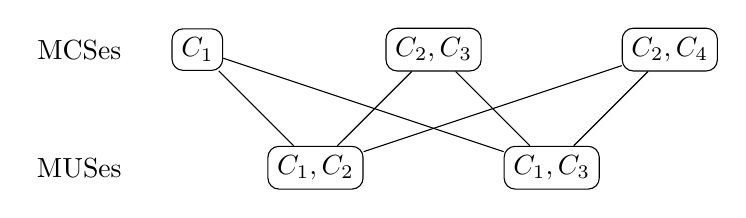
\begin{tikzpicture}[scale=1.5, 
				    state/.style={draw, rounded corners, fill=none,
				    			  text centered, text=black}]
	\node[] (u0) at (1, 2) {MCSes};
	\node[state] (u1) at (2, 2) {$C_{1}$};
	\node[state] (u2) at (4, 2) {$C_{2}, C_{3}$};
	\node[state] (u3) at (6, 2) {$C_{2}, C_{4}$};
	\node[state] (u4) at (3, 1) {$C_{1}, C_{2}$};
	\node[state] (u5) at (5, 1) {$C_{1}, C_{3}$};
	\node[] (u6) at (1, 1) {MUSes};
	
	\path[-] 	(u1)  edge   (u4);
	\path[-] 	(u1)  edge   (u5);
	\path[-] 	(u2)  edge   (u4);
	\path[-] 	(u2)  edge   (u5);
	\path[-] 	(u3)  edge   (u4);
	\path[-] 	(u3)  edge   (u5);

\end{tikzpicture}

	\end{center}
	\caption{Duality of MUSs and MCSs.}
	\label{fig:graph}
\end{figure}

\begin{example}
		To illustrate this duality we use our example formula: $$\varphi=\underbrace{(x)}\limits_{C_{1}}\wedge\underbrace{(\neg x)}\limits_{C_{2}}\wedge\underbrace{(\neg x\vee y)}\limits_{C_{3}}\wedge\underbrace{(\neg x \vee \neg y)}\limits_{C_{4}}$$ First, the set of MCSs of $\varphi$  $\{\{C_{1}\}, \{C_{2}, C_{3}\}, \{C_{2}, C_{4}\}\}$, whose minimal hitting sets are $\{\{C_{1}, C_{2}\}, \{C_{1}, C_{3,} C_{4}\}\}$ which is exactly the set of MUSs (given in Table \ref{mus-mcs}). Similarly, we can show that the set of MCSs is the set of minimal hitting sets of the set of MUSSs. So, every MCS has at least one clause from every MUS and vice-versa. The duality is illustrated in Figure \ref{fig:graph}.
	
\end{example}
\subsection{AtMost Constraints}
 An AtMost Constraint states that the number of the literals from a given set does not exceed a given upper bound. For $\{l_{1}, l_{2}, l_{3},\cdots ,l_{\text n}\}$ being a set of $n$ literals and $k$ a non-negative integer, the corresponding AtMost constraint is defined as:
$$AtMost(\{l_{1},l_{2},\ldots,l_{n}\},k)\equiv \sum\limits^{n}_{i=1} val(l_{i})\leqslant k$$
where $val(l_{\text i})$ is 1 if $l_{i}$ is assigned $\mathbf{true}$ and otherwise 0.The bound $k$ tells that at most how many literals can be assigned $]\mathbf{true}$.\newline
the authors used an implementation of the AtMost constraints where the variables are watched and propagates the negation of each literal when $k$ of them are assigned $\mathbf{true}$. This is implemented with exactly $n$ watched literals and a counter that is incremented or decremented whenever one of them is assigned or unassigned.
\begin{example}
Consider formula $\varphi = (l_{1}\vee l_{2}\vee l_{3})$ with the AtMost constraint $\varphi_{AM}=AtMost(\{l_{1}\vee l_{2}\vee l_{3}\}, 2)$. Solving the formula $\varphi
\wedge \varphi_{AM}$ might assign $\mathbf{true}$ to $l_{1}$ and $l_{2}$, but $\varphi_{AM}$ will assure that $l_{3}$ will be assigned $\mathbf{false}$.
\end{example}
